\documentclass[border=3pt]{standalone}
% Preâmbulo compartilhado pelos diagramas TikZ da aula 7 (Filtros Não Paramétricos)
\usepackage[T1]{fontenc}
\usepackage[utf8]{inputenc}
\usepackage{lmodern}
\usepackage{amsmath}
\usepackage{xcolor}
\usepackage{tikz}
\usetikzlibrary{arrows.meta,angles,quotes,decorations.pathmorphing,calc,
                positioning,shapes.geometric,shapes.misc,backgrounds,fit,
                math}

% Paleta (mesma dos SVGs originais)
\definecolor{dblue}{HTML}{2A5B8C}
\definecolor{dorange}{HTML}{B3541E}
\definecolor{dgreen}{HTML}{4A7C59}
\definecolor{dred}{HTML}{9C4B4B}
\definecolor{dcream}{HTML}{F4F1EA}
\definecolor{dshade}{HTML}{DDD7C9}

% Função gaussiana (não normalizada por padrão de escala visual)
\pgfmathdeclarefunction{gauss}{3}{%
  \pgfmathparse{1/(#3*sqrt(2*pi))*exp(-((#1-#2)^2)/(2*#3^2))}%
}

% Estilos comuns (prefixo d... para não colidir com chaves internas do pgf)
\tikzset{
  >={Stealth[length=2mm]},
  dguide/.style={gray!55, dashed, line width=0.4pt},
  daxis/.style={gray!60, line width=0.7pt, ->},
  dbody/.style={fill=black!3, draw=black!80, line width=1pt},
  dacc/.style={draw=dblue, line width=1pt},
  dlbl/.style={black!55, font=\small},
  dsub/.style={black!45, font=\footnotesize},
  dstate/.style={circle, draw=black!80, fill=dcream, line width=1pt,
                 minimum size=17mm, font=\large, inner sep=1pt},
  dobs/.style={circle, draw=black!80, fill=dshade, line width=1pt,
               minimum size=14mm, font=\large, inner sep=1pt},
  dbox/.style={rounded corners=2pt, draw=black!80, fill=dcream, line width=1pt,
               align=center, inner sep=6pt},
  dop/.style={circle, draw=black!80, fill=white, line width=1pt,
              minimum size=6mm, inner sep=0pt, font=\small},
  dtrans/.style={->, dblue, line width=1pt},
  dmeas/.style={->, dorange, line width=1pt},
  dcurve/.style={line width=1pt, dblue},
  dcurveb/.style={line width=1.4pt, dorange},
}

\begin{document}
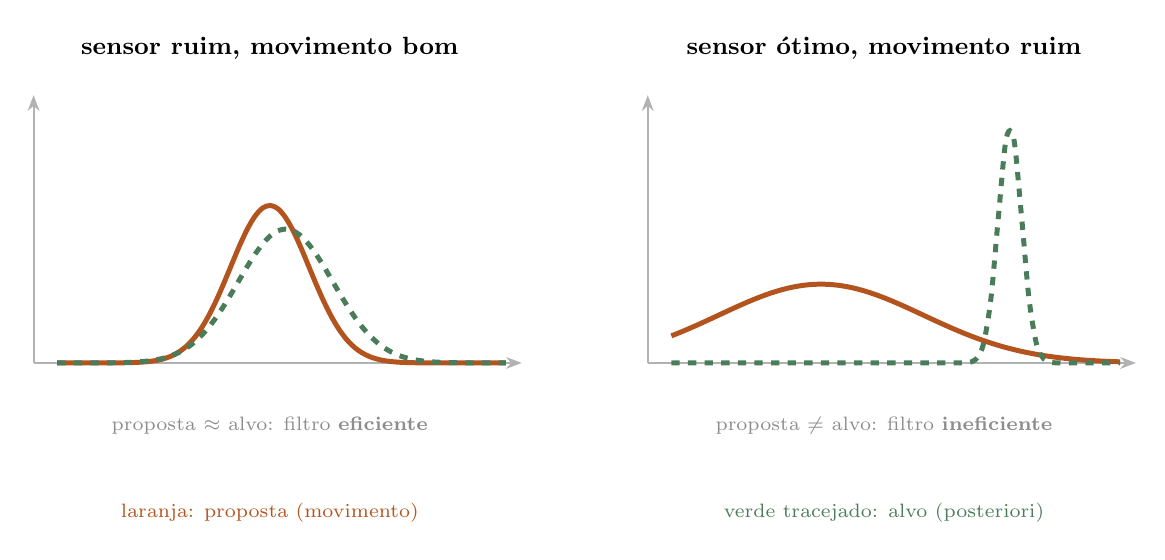
\begin{tikzpicture}[x=1cm,y=1cm]
  \newcommand{\painel}[2]{\begin{scope}[shift={(#1)}] \draw[daxis] (0,0) -- (6.2,0); \draw[daxis] (0,0) -- (0,3.4); \node[font=\small\bfseries] at (3,4.0) {#2};}
  \painel{0,0}{sensor ruim, movimento bom}
  \draw[dorange, line width=1.8pt, domain=0.3:6, samples=60, smooth] plot (\x, {2.0*exp(-((\x-3)*(\x-3))/(2*0.5*0.5))});
  \draw[dgreen, line width=1.8pt, dashed, domain=0.3:6, samples=60, smooth] plot (\x, {1.7*exp(-((\x-3.2)*(\x-3.2))/(2*0.6*0.6))});
  \node[dsub, font=\scriptsize, align=center] at (3,-0.8) {proposta $\approx$ alvo: filtro \textbf{eficiente}};
  \end{scope}
  \painel{7.8,0}{sensor ótimo, movimento ruim}
  \draw[dorange, line width=1.8pt, domain=0.3:6, samples=60, smooth] plot (\x, {1.0*exp(-((\x-2.2)*(\x-2.2))/(2*1.3*1.3))});
  \draw[dgreen, line width=1.8pt, dashed, domain=0.3:6, samples=60, smooth] plot (\x, {3.0*exp(-((\x-4.6)*(\x-4.6))/(2*0.15*0.15))});
  \node[dsub, font=\scriptsize, align=center] at (3,-0.8) {proposta $\ne$ alvo: filtro \textbf{ineficiente}};
  \end{scope}
  \node[dorange, font=\scriptsize] at (3.0,-1.9) {laranja: proposta (movimento)}; \node[dgreen, font=\scriptsize] at (10.8,-1.9) {verde tracejado: alvo (posteriori)};
\end{tikzpicture}
\end{document}
